\documentclass[]{article}
\usepackage{graphicx}
\usepackage{indentfirst}
\usepackage{amsmath}
\usepackage{clrscode3e}
\setlength{\parindent}{0pt}


\title{HW06 for ECE 9343}
\author{Tongda XU, N18100977}

\begin{document}

\maketitle

\section{Question 1: Huffman Code Running}
One possible result:\\
\{ h: 00, a: 11, b: 100, f:101, d: 110, e: 1111, c: 11100, g: 11101 \} 

\section{Question 2: CLRS Problem Set 16.1}
\subsection{Describe a greedy algorithm}

\begin{codebox}
	
	\Procname{$\proc{CC($k$)}$}
	\li $Change \leftarrow \{25, 10, 5, 1\}$
	\li $Result \leftarrow []$
	\li \For each c in $Change$
	\li 	\Do $Result [c] = \proc{floor($k/c)$}$
	\li     $k = k \mod c$  \End  
	\li \Return $Result$
\end{codebox}

Suppose that we are working with coin set \{30, 10, 5, 1\}, it is fairly easy to find out that in any step of loop 3-5, if we did not select the greedy choice, which is let the current largest coin fill result first, the reminder would be larger than the current largest coin. Since the largest coin could be divided by the second largest one, the reminder needs at lease $\frac{largest}{second largest}$ coin to fill the reminder, which could be merged into at least 1 largest coin to reduce number of coins.\\

For the case of \{25, 10, 5, 1\} it becomes tricky. the larger than 30 case could be easily cut into 25 and 5, which is obviously better than 3*10. But for \{26, 27, 28, 29\}, we have to enumerate this four case to proof, such that 26 = 25 + 1 = 2*10 + 5 + 1, 27 = 25 + 1 + 1 = 2*10 + 5 + 1 + 1, 28 = 25 + 3*1 = 2*10 + 5 + 3*1, 29 = 25 + 4*1 = 2*10 + 5 + 4*1 to complete the proof. 

\subsection{Proof greedy works for power sequence}

Suppose that in any step of loop 3-5, the reminder $r$ is larger than divider $c_i$, which is not the greedy choice, then it is easy to find out that $r$ requires at least c times $c_{i-1}$, or $c^2$ times $c_{i-2}$, which could be merged into 1 $c_i$ to reduce the number of coins.

\subsection{Describe a set of coins greedy does not apply}
Consider =\{4, 3, 1\} dividing 6

\subsection{Describe a universal (DP) solution}

\begin{codebox}
	
	\Procname{$\proc{CC($n$)}$}
	\li $DP \leftarrow []$
	\li $Change \leftarrow \{k_k, ..., k_1\}$
	\li \Return \proc{CC-Aid($n$)}

\end{codebox}

\begin{codebox}
	
	\Procname{$\proc{CC-Aid($k$)}$}
	\li \If $DP[k] \neq NIL$
	\li \Then \Return $DP[k]$
	\li \Else
	\li $DP[k] \leftarrow \underset{k_i \in Change, k-k_i \ge 0 }{\min} \{\proc{CC-Aid($n-k_i$)}\} + 1$
	\li \Return $DP[k]$
	
\end{codebox}

This algorithm construct a dictionary of size n, and each time rely on the retrieve of previous k element in total of O(n) time, thus the running time would be O(k + nk) = O(nk). 

\section{Question 3: CLRS Exercise 15.4-3}

See Figure \ref{fig:6_Prism}

\begin{figure}
	\centering
	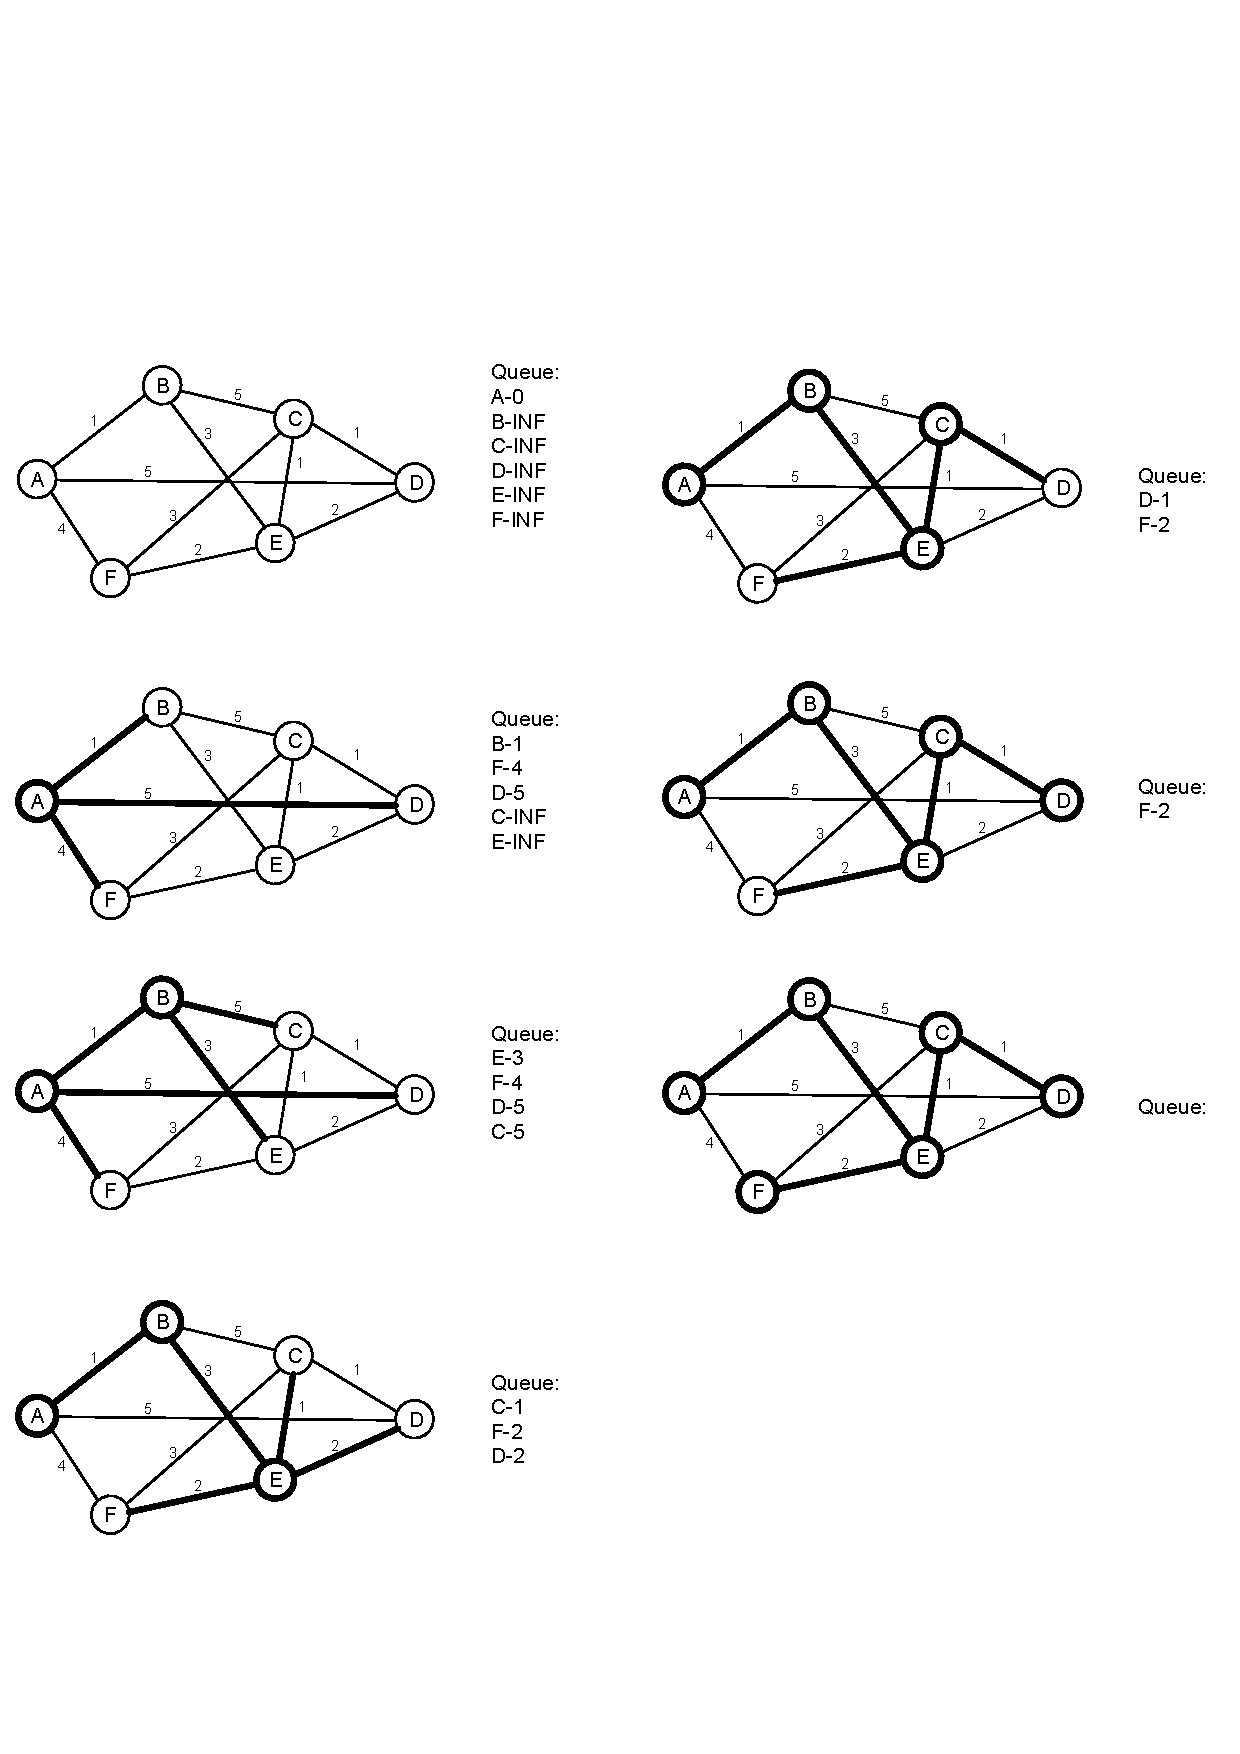
\includegraphics[width=\linewidth]{6_Prism}
	\caption{Prism algorithm running procedure}
	\label{fig:6_Prism}
\end{figure}

\end{document}
